\chapter{Results}

XXXXXXXXXXXXXXXXX

\section{Tables and graphics}

XXXXXXXXXXXXXXXXX

\begin{figure}[!ht]
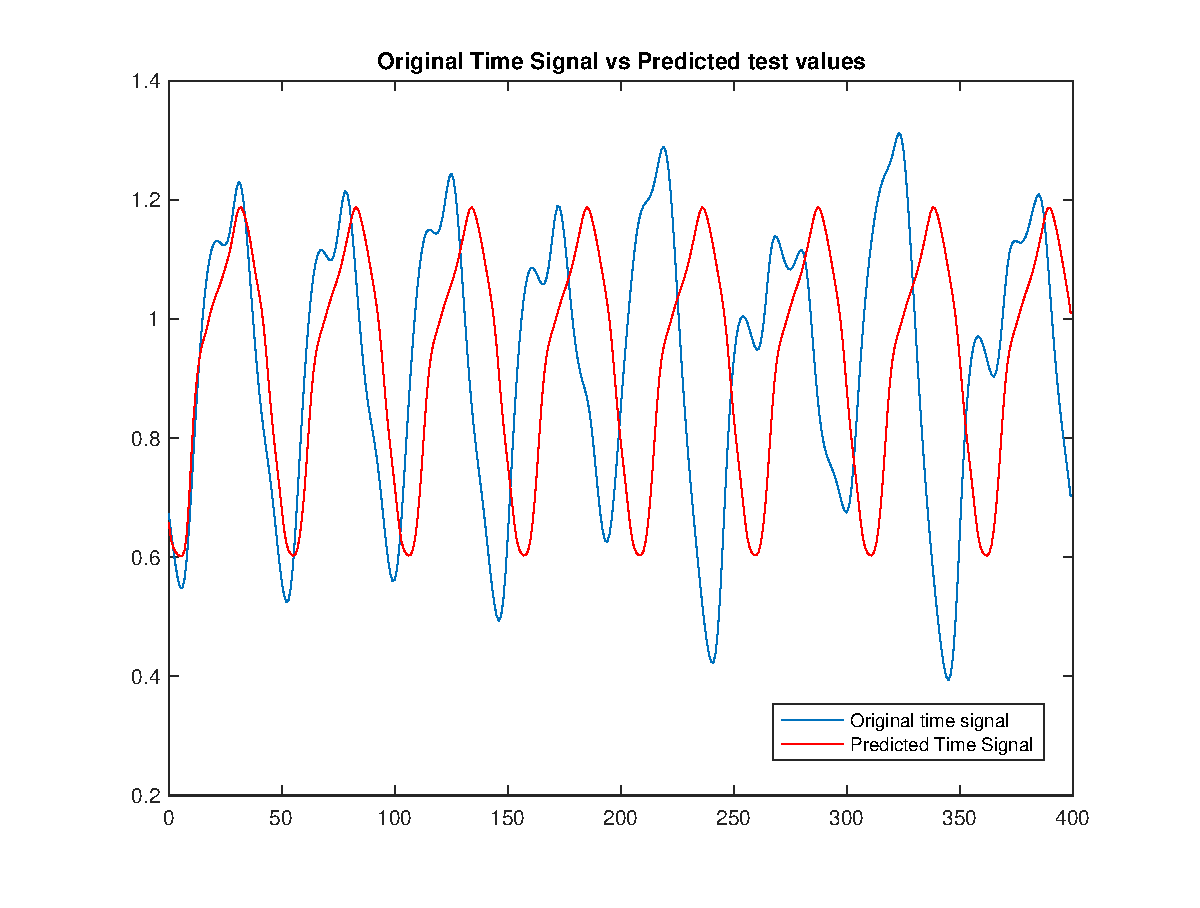
\includegraphics[clip,width=\columnwidth]{figures/PlotTimeSeriesResult}% 
\caption{This is an example of a figure and its caption.}
\label{fig:timeseries}
\end{figure}

\begin{table}[!ht]
\renewcommand{\arraystretch}{1.50}
\caption{This is an example of a table and its caption.}
\label{tablePCA}
\centering
\begin{tabular}{| c | c |}
\hline
\bfseries PCA & \bfseries Residual mean (in absolute values) \\
\hline\hline
Original PCA & 0.1267  \\
\hline
PCA on Centroid 1 & 0.1249\\
\hline
PCA on Centroid 2 & 0.1214  \\
\hline
\end{tabular}
\end{table}

\newpage


